\subsection{Szintillationsdetektor}
\begin{figure}
\centering
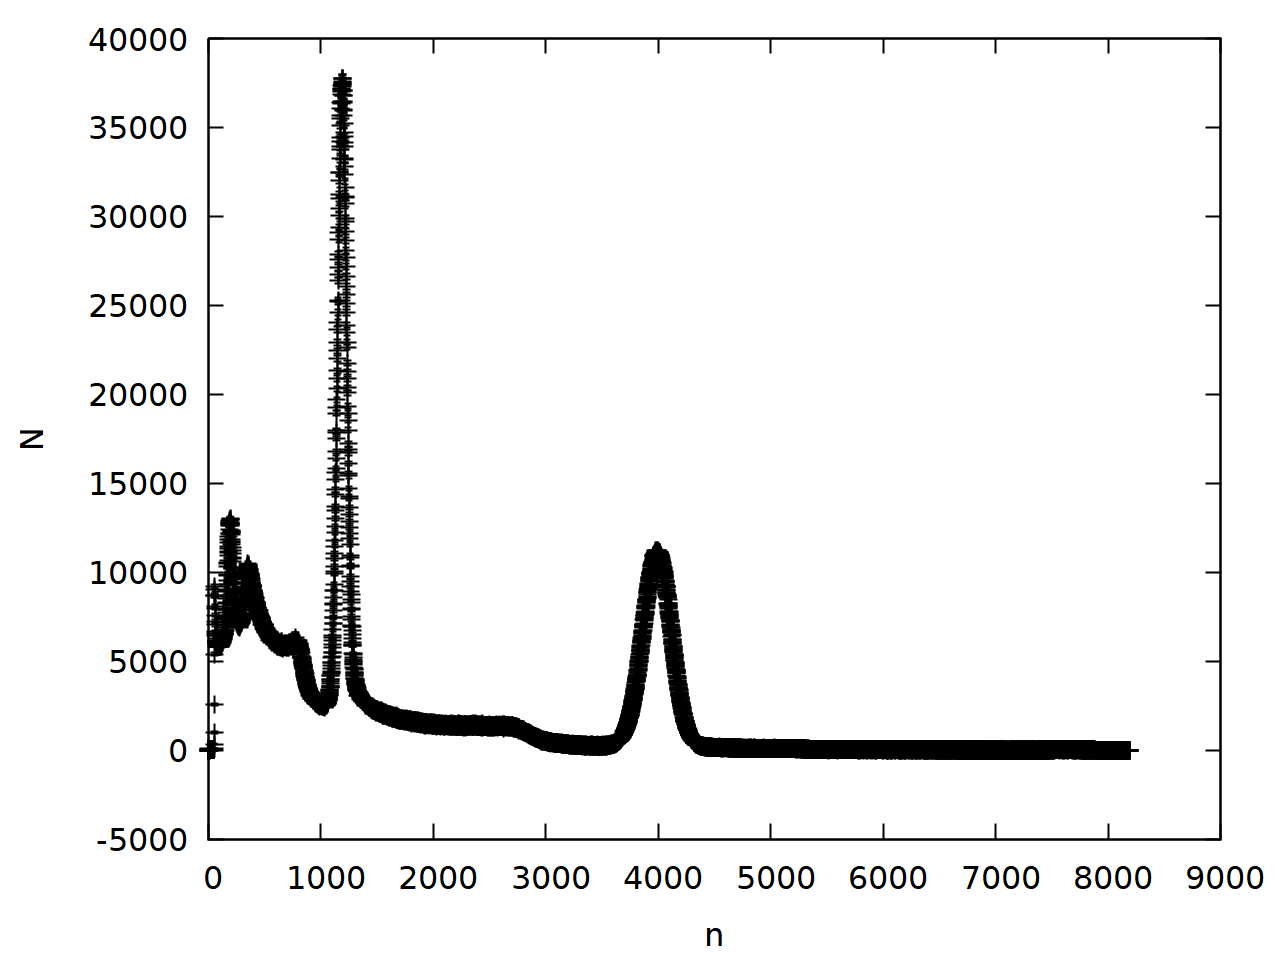
\includegraphics[width=0.7\linewidth]{data/si_cs.png}
\caption{Szintillator Cs korrigiert}
\label{fig:si_cs}
\end{figure}

\begin{figure}
\centering
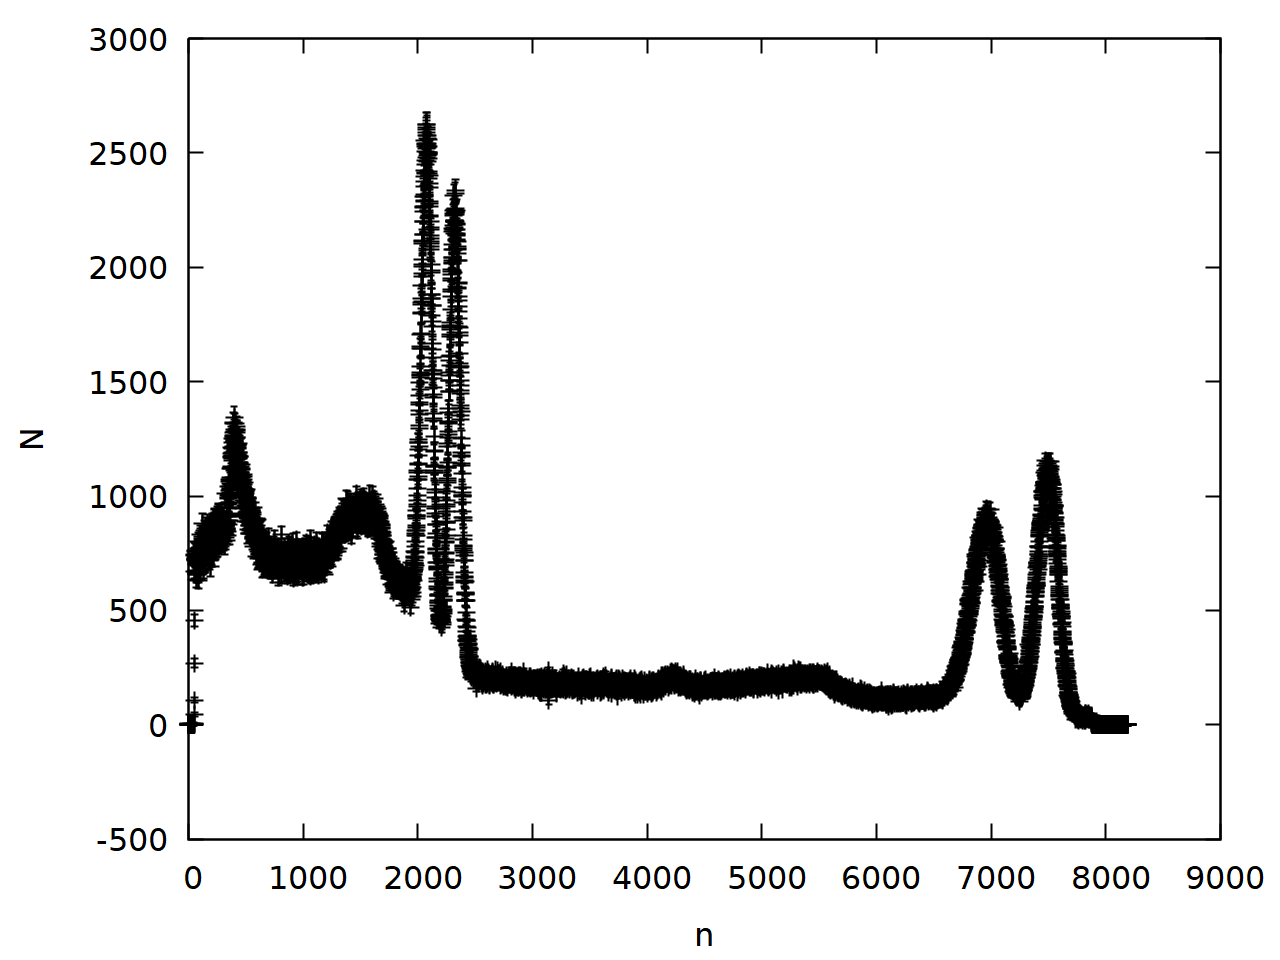
\includegraphics[width=0.7\linewidth]{data/si_co.png}
\caption{Szintillator Co korrigiert}
\label{fig:si_co}
\end{figure}

\begin{figure}
\centering
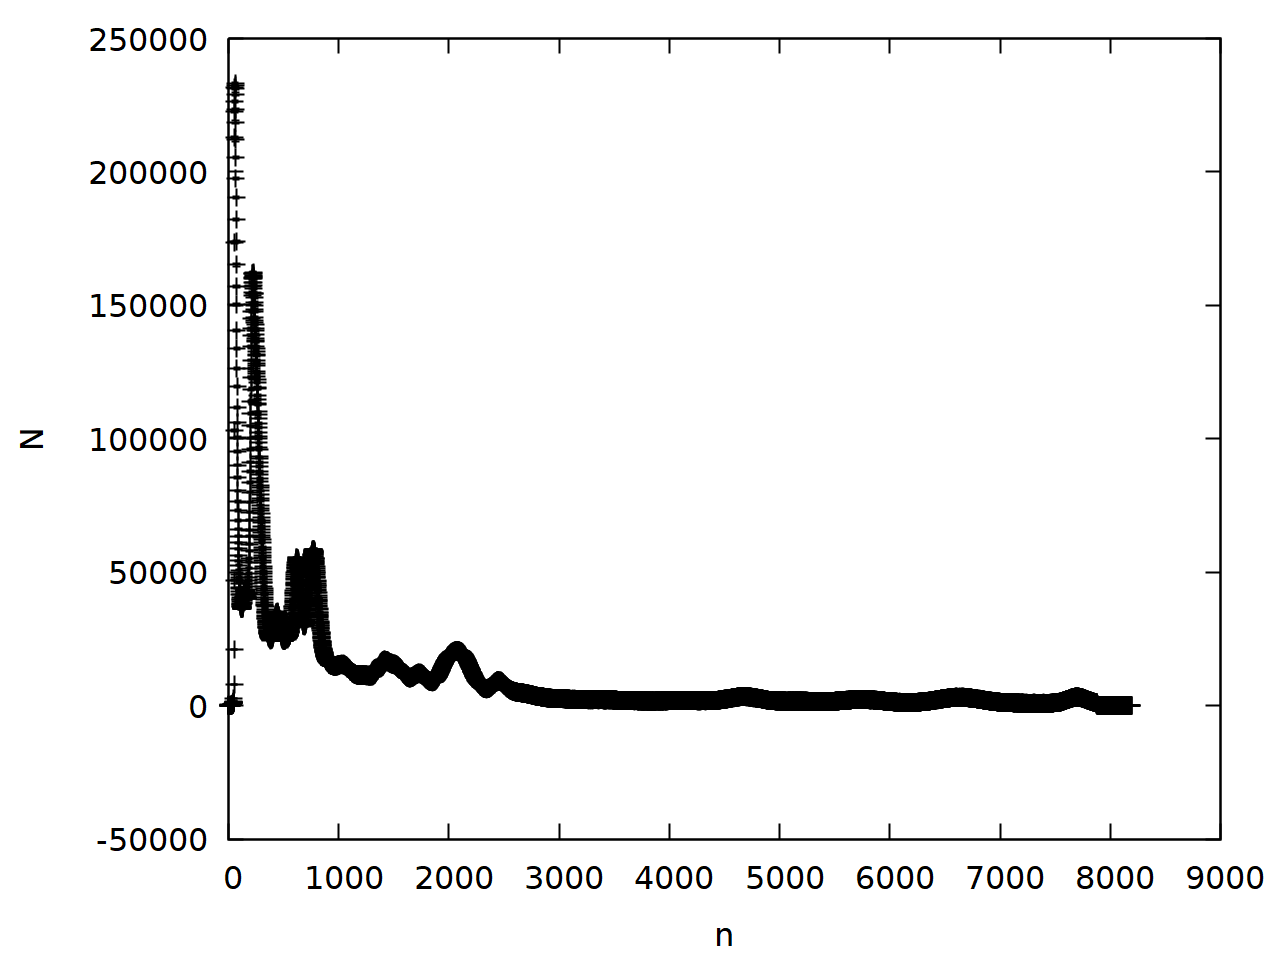
\includegraphics[width=0.7\linewidth]{data/si_eu.png}
\caption{Szintillator Eu korrigiert}
\label{fig:si_eu}
\end{figure}

Die aufgenommenen Spektren im Anhang werden um den Untergrund korrigiert (Werte kleiner 0 werden auf 0 gesetzt) und sind in Abbildung \ref{fig:si_cs} - \ref{fig:si_eu} abgebildet. Als Fehler wird $\sqrt{N}$ angenommen. An die stärksten Linien der 3 Spektren werden nun Gausskurven gefittet\[f(x) = a\exp{\left(-4\ln{2}\frac{(x-b)^2}{\text{FWHM}^2}\right)}\]. Das Ergebnis ist in Tabelle \ref{tab:si} abgebildet (die Halbwertsbreite wurde schon auf keV umgerechnet).

\begin{table}
\caption{Fitergebnisse an den Spektren des Szintillators}
\begin{tabular}{cccccccccc}
\toprule
Peak Nr. & Element & Energie/\si{keV}& $a$ & $\Delta a$ & $b$ & $\Delta b$ & FWHM/\si{keV} & $\Delta \text{FWHM}/\si{keV}$\\
\midrule 
1	&	Cs	&	661,66	&	37781	&	933	&	1193	&	0,9	&	57	&	3\\
2	&	Co	&	1332,5	&	2586	&	90	&	2068	&	1,9	&	82	&	5\\
3	&	Co	&	1173,2	&	2301	&	94	&	2323	&	1,9	&	68	&	4\\
4	&	Eu	&	121,7825	&	160500	&	3181	&	234	&	0,9	&	69	&	4\\
5	&	Eu	&	344,281	&	53500	&	2255	&	610	&	1,8	&	55	&	4\\
6	&	Eu	&	1408,011	&	21300	&	691	&	2055	&	4,9	&	221	&	13\\
\bottomrule
\end{tabular}
\label{tab:si}
\end{table}

Um den Linien die Energie zuzuordnen wurde zuerst der Cäsiumpeak bestimmt. Für Cäsium war uns nur eine Linie (\SI{662}{keV}) vorgegeben. Leider gibt es 2 verschiedene Peaks im Spektrum. Um zu bestimmen, welcher der beiden Peaks der richtige ist, haben wir jeweils den Umrechnungsfaktor Kanal $\leftrightarrow$ Energie abgeschätzt und dann die Energien der restlichen Peaks bestimmt. Bei dem linken Peak gab es eine deutlich bessere Übereinstimmung, so dass wir davon ausgehen, dass dieser Peak der \SI{662}{keV} ist.\\
Um den Umrechnungsfaktor Kanal $\leftrightarrow$ Energie zu bestimmen, tragen wir die Kanalnummer über der Energie der Peaks auf und führen einen linearen Fit \[f(x) = C\ind{Si}\cdot x\] durch (siehe Abbildung \ref{fig:si_gauge}). Als Fehler der Kanalnummer nehmen wir die Standartweichung der Gausskurve an. Der Fit ergibt: $C\ind{Si} = \si{(1,77\pm 0,09)\,Kanal/keV}$

\begin{figure}
\centering
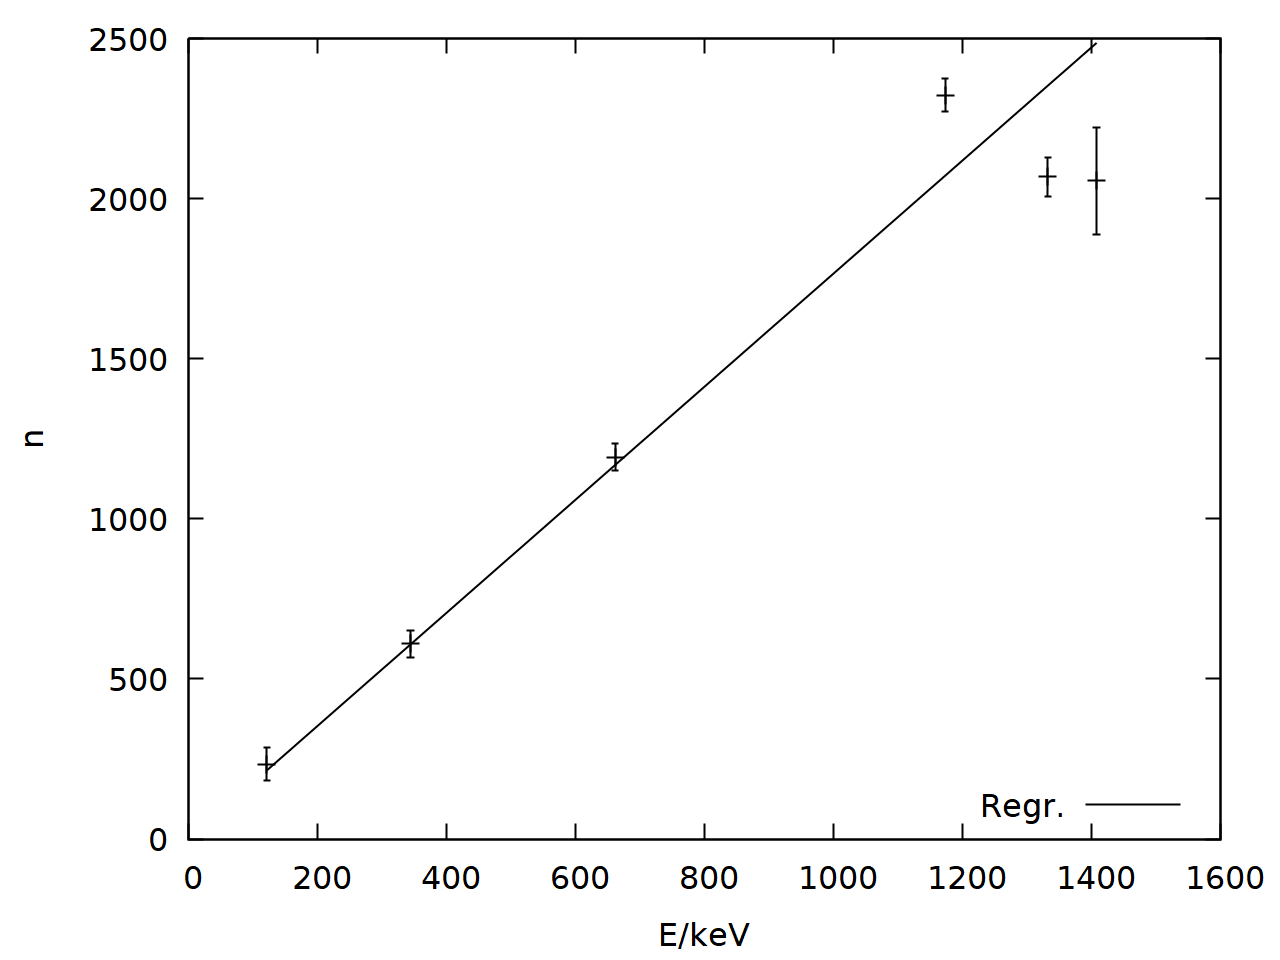
\includegraphics[width=0.7\linewidth]{data/si_gauge.png}
\caption{Szintillator Kalibrierung}
\label{fig:si_gauge}
\end{figure}

\subsubsection*{Peak-to-Total}
Die gesamte Anzahl der untergrundkorrigierten Ereignisse beträgt für Cäsium: $N\ind{total}\upd{Cs} = 17152004 \pm 4141$ und für Cobalt: $N\ind{total}\upd{Co} = 3482320\pm 1866$ (Als Fehler wurde wieder $\sqrt{N}$ angenommen). 
Um die Anzahl der Ereignisse in den Peaks unabhängig vom Kontinuum abzuschätzen, berechnen wir die Fläche unter der jeweiligen Gausskurve \[N\ind{Peak} = a\cdot\sqrt{2\pi}\cdot \sigma\], wobei $\sigma$ die Standartabweichung der Gausskurve ist.
Damit ergibt sich für den Cs-Peak: $\text{PtT}\upd{Cs} = \cfrac{N\ind{Peak}\upd{Cs}}{N\ind{total}\upd{Cs}} = 0,237\pm 0,007$ und die beiden Cobaltpeaks (diese werden nach Praktikumsanleitung zusammenaddiert): $\text{PtT}\upd{Co} = 0,198\pm 0,007$.

\subsection{Halbleiter-Detektor}
\begin{figure}
\centering
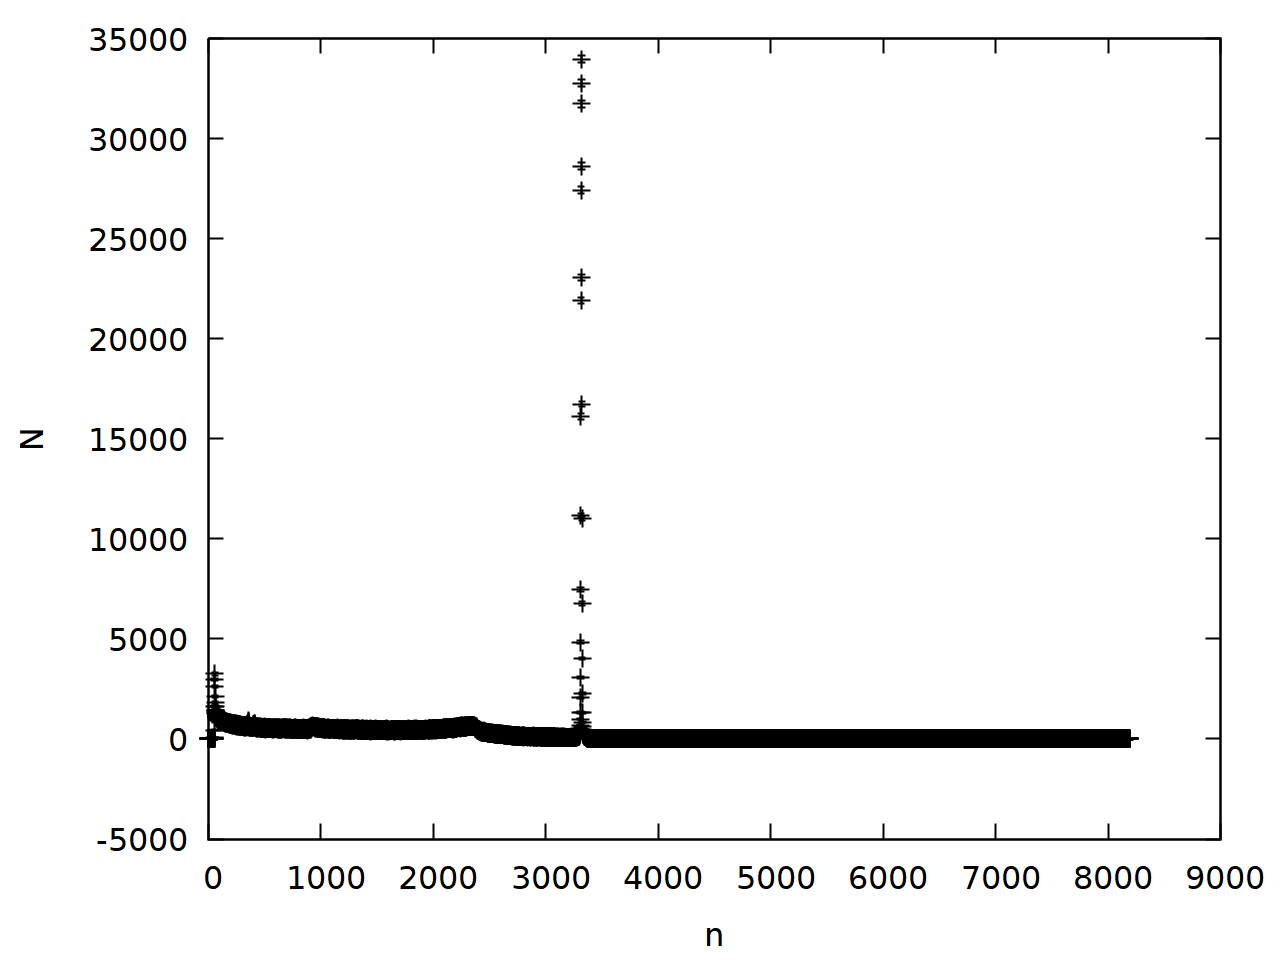
\includegraphics[width=0.7\linewidth]{data/ge_cs.png}
\caption{Halbleiter Cs korrigiert}
\label{fig:ge_cs}
\end{figure}

\begin{figure}
\centering
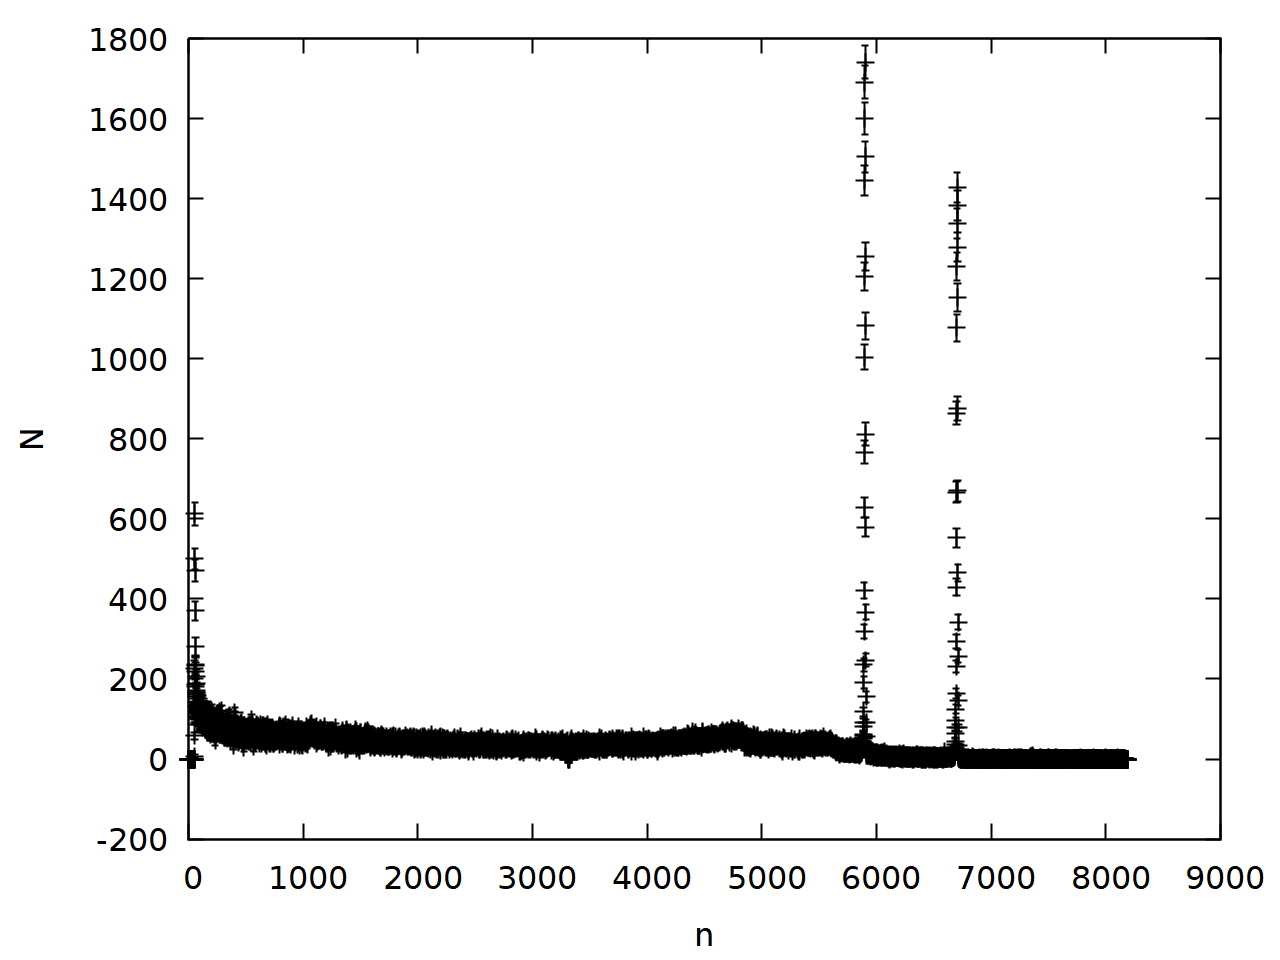
\includegraphics[width=0.7\linewidth]{data/ge_co.png}
\caption{Halbleiter Co korrigiert}
\label{fig:ge_co}
\end{figure}

\begin{figure}
\centering
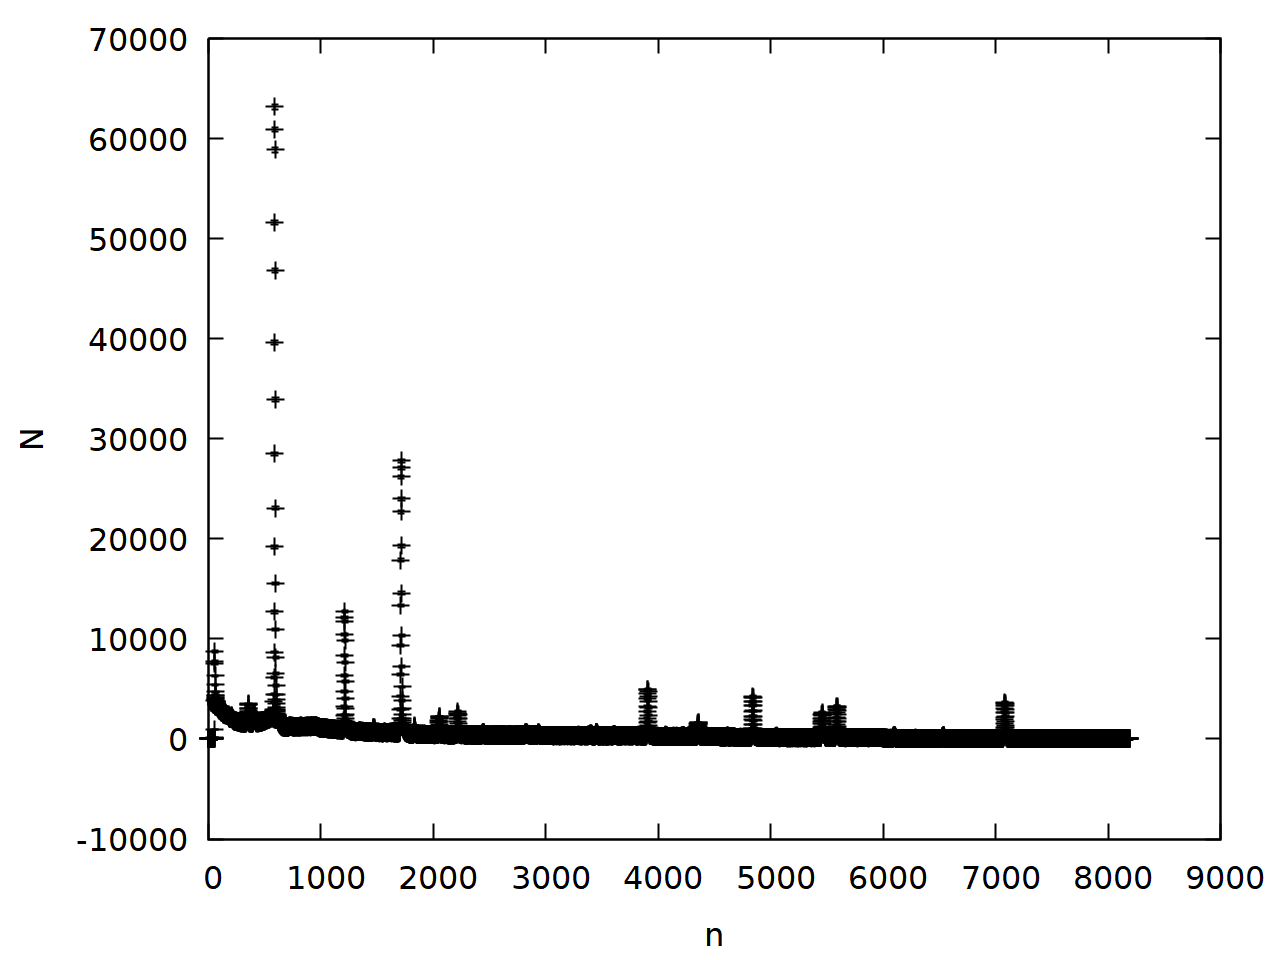
\includegraphics[width=0.7\linewidth]{data/ge_eu.png}
\caption{Halbleiter Eu korrigiert}
\label{fig:ge_eu}
\end{figure}

Die Auswertung des Halbleiterdetektors geschieht analog zur Auswertung des Szintillators. In den Abbildungen \ref{fig:ge_cs} - \ref{fig:ge_eu} sind die gemessenen Spektren der Proben abgebildet. Wieder werden Gausskurven an die Peaks gefittet (siehe Tabelle \ref{tab:ge}). Die Zuordnung des Cäsiumpeaks ist bei diesem Detektor einfacher, weil sich nur ein Peak im Bereich befindet. Vergleicht die Form des Spektrums in der Umgebung des Peaks, so kann man erkennen, dass es sich um den gleichen Peak wie beim Szintillator handelt.\\

\begin{table}
\caption{Fitergebnisse an den Spektren des Halbleiterdetektor}
\begin{tabular}{cccccccccc}
\toprule
Peak Nr. & Element & Energie/\si{keV}& $a$ & $\Delta a$ & $b$ & $\Delta b$ & FWHM/\si{keV} & $\Delta \text{FWHM}/\si{keV}$\\
\midrule 
1	&	Cs	&	661,66	&	32170	&	796	&	3316,9	&	0,1	&	1,68	&	0,03\\
2	&	Co	&	1173,2	&	1596	&	77	&	5899,8	&	0,2	&	2,06	&	0,06\\
3	&	Co	&	1332,5	&	1427	&	63	&	6704,0	&	0,2	&	1,79	&	0,06\\
4	&	Eu	&	121,78	&	56415	&	11932	&	591,8	&	0,6	&	1,56	&	0,23\\
5	&	Eu	&	244,6989	&	10944	&	5376	&	1212,9	&	1,5	&	1,61	&	0,59\\
6	&	Eu	&	344,281	&	25549	&	7567	&	1715,2	&	0,9	&	1,73	&	0,35\\
7	&	Eu	&	778,903	&	4691	&	3072	&	3908,0	&	2,4	&	1,99	&	0,97\\
8	&	Eu	&	964,131	&	4056	&	2667	&	4843,0	&	2,6	&	2,19	&	1,05\\
9	&	Eu	&	1085,914	&	2527	&	2133	&	5458,0	&	3,5	&	2,19	&	1,42\\
10	&	Eu	&	1112,116	&	3121	&	2389	&	5590,0	&	3,2	&	2,19	&	1,26\\
11	&	Eu	&	1408,011	&	3655	&	2361	&	7084,0	&	2,8	&	2,39	&	1,08\\
\bottomrule
\end{tabular}
\label{tab:ge}
\end{table}

Nachdem man den Peaks die Energien zugeordnet hat, wird wieder zur Kalibration der Kanal über der Energie aufgetragen (siehe Abbildung \ref{fig:ge_gauge}). Ein linearer Fit ergibt: $C\ind{Ge} = \si{(5,025\pm 0,004)\,Kanal/keV}$

\begin{figure}
\centering
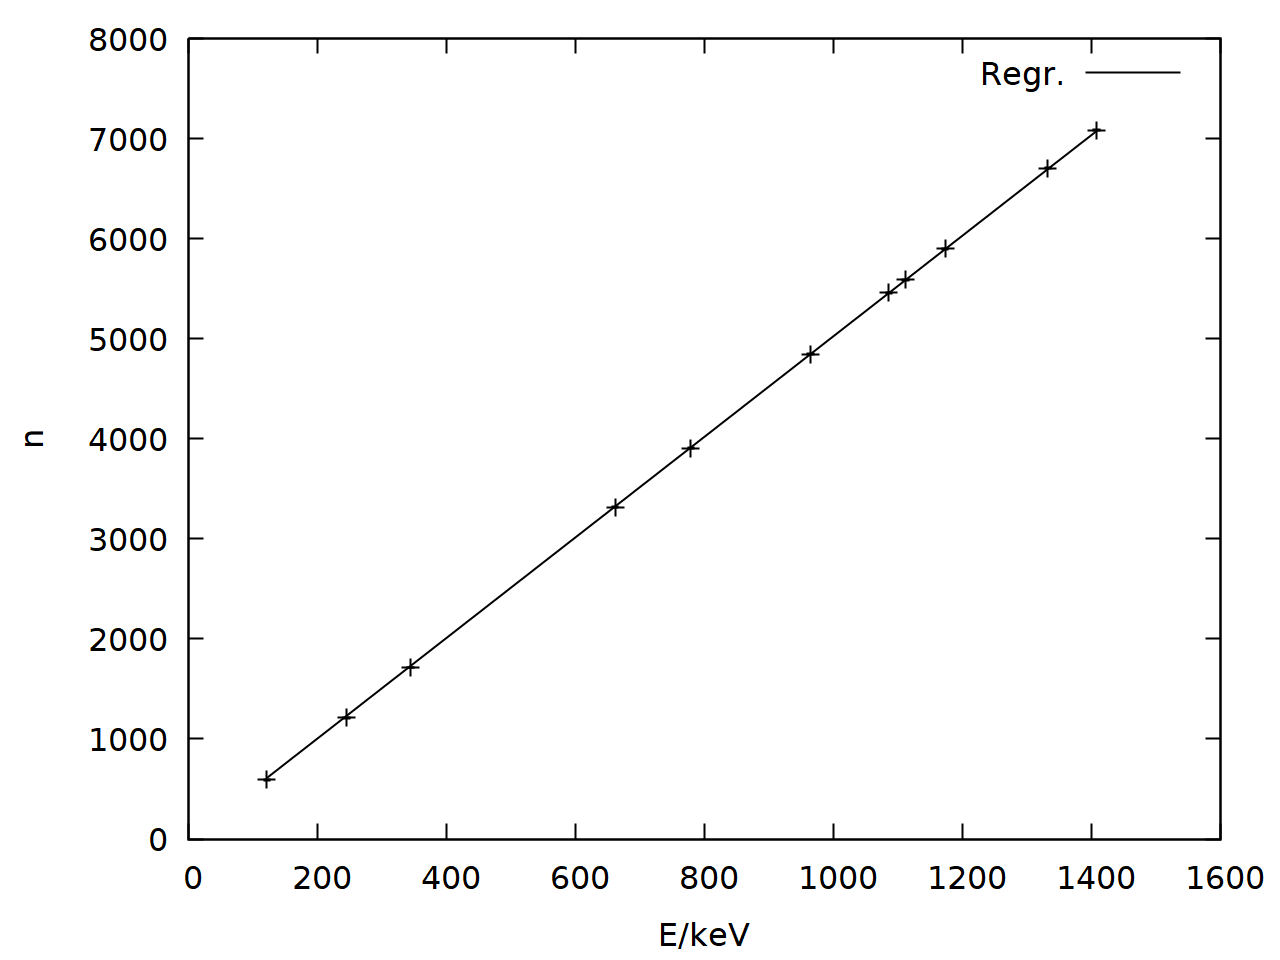
\includegraphics[width=0.7\linewidth]{data/ge_gauge.png}
\caption{Halbleiter Kalibrierung}
\label{fig:ge_gauge}
\end{figure}

\subsubsection*{Peak-to-Total}
Die gesamte Anzahl der untergrundkorrigierten Ereignisse beträgt für Cäsium: $N\ind{total}\upd{Cs} = 1762931 \pm 1328$ und für Cobalt: $N\ind{total}\upd{Co} = 304614\pm 552$.\\
Damit ergibt sich für den Cs-Peak: $\text{PtT}\upd{Cs} = 0.163\pm 0,005$ und die beiden Cobaltpeaks: $\text{PtT}\upd{Co} = 0.103\pm 0,004$. Das PtT-Verhältnis ist also für den Halbleiter kleiner als für den Szintillator.